%MIT OpenCourseWare: https://ocw.mit.edu
%RES.18-011 Algebra I Student Notes, Fall 2021
%License: Creative Commons BY-NC-SA 
%For information about citing these materials or our Terms of Use, visit: https://ocw.mit.edu/terms.

\section{The Icosahedral Group}

\subsection{Review: The Class Equation}
Last time, we discussed the conjugacy class of an element, which is the orbit of an element under conjugation, and the centralizer of an element, which is the stabilizer of an element under conjugation. 
\begin{definition}
The \textbf{conjugacy class} of an element is 
\[
C(x) \coloneqq \{gxg^{-1} : g \in G\} \subseteq G.
\]
\end{definition}

\begin{definition}
The \textbf{centralizer} of an element is 
\[
Z(x) \coloneqq \{g: gxg^{-1} = x\} \leq G.
\]
\end{definition}

The \textbf{class equation} states that 
\[
|G| = |C_1| + \cdots + |C_k|,
\]
which tells us information about a group simply through numerics.

\subsection{Basic Information}
The group $I \leq SO_3$ is the icosahedral group, which is the group of symmetries of the icosahedron under rotations (orientation-preserving isometries in $\RR^3$.) It is isomorphic to the dodecahedral group.

The group is \[I = \{\rho_{(u, \theta)}\},\] where each $\rho_{(u, \theta)}$ is a rotation by $\theta$ around a vector $u$ preserved by the rotation, which is called a \emph{pole} of $u.$ Additionally, the rotations have the property that $\rho_{(u, \theta)} = \rho_{(-u, -\theta)}.$ For a polyhedral group, $u$ lies on a face, an edge, or a vertex of the polyhedron. 

Let's start with counting the number of rotations in $I$ by whether the pole is on a face, an edge, or a vertex.

\begin{center}
    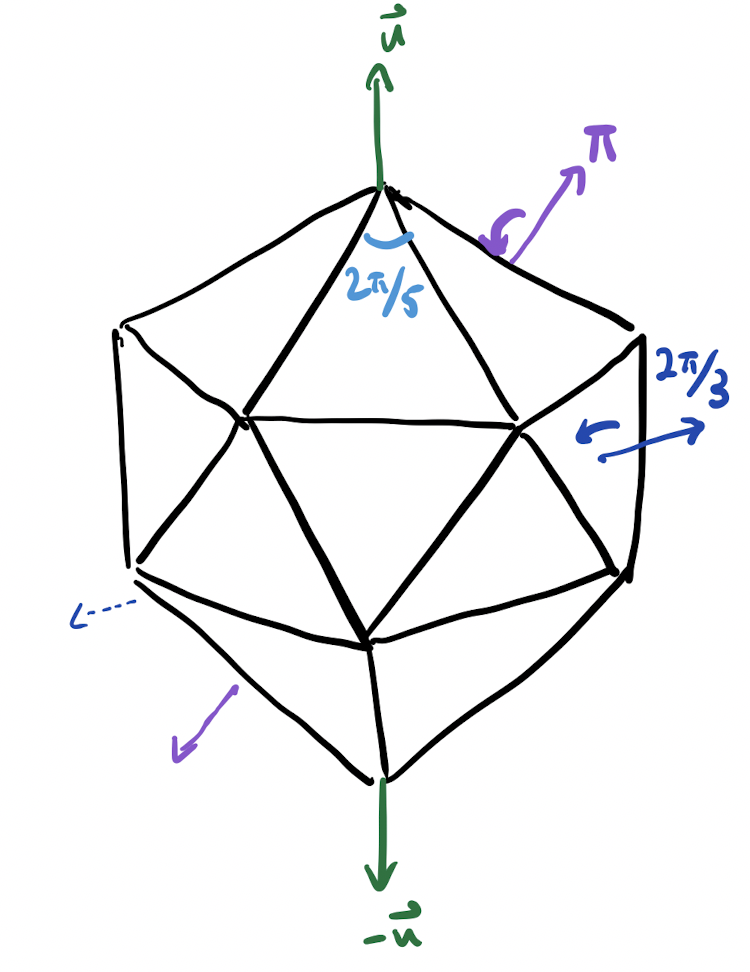
\includegraphics[width=7cm]{Lecture Files and Images/lec20-icos.png}
\end{center}

\begin{itemize}
    \item \textbf{Identity.} The trivial rotation is one rotation. 
    \item \textbf{20 faces.} For each face, excluding the identity, there are 2 rotations by $2\pi/3$ and $4\pi/3,$ which is 40 rotations total. In this way, every rotation is counted twice, since $\rho_{(u, \theta)} = \rho_{(-u, \theta)},$ 
    and every pole through the center of a face also goes through the opposite face. So we count 20 face rotations total.
    
    \item \textbf{30 edges.} For each face, there is one (non-identity) rotation by $\pi,$ and this also gets double-counted, so there are $30/2 = 15$ edge rotations total. 
    
    \item \textbf{12 vertices.} For each vertex, there are four nontrivial rotations, by $2\pi/5, 4\pi/5, 6\pi/5,$ and $8\pi/5.$ This double-counts as well, so there are $12 \cdot 4 / 2 = 24$ total vertex rotations.
\end{itemize}

In total, we have $1 + 20 + 15 + 24 = 60$ rotations. 
\subsection{Conjugacy Classes}

Now, it is possible to understand $I$ by thinking about the group action of conjugation on itself.
\begin{qq}
How can we decompose $I$ into conjugacy classes and what does the class equation tell us about normal subgroups of $I$? 
\end{qq}

For $g \in I,$ the conjugate of $\rho_{(p, \theta)}$ under $g$ is $g\rho_{(p, \theta)} g^{-1} = \rho_{(q, \theta)}$, where $q = g(p),$ since conjugating by $g$ is essentially taking a change of coordinates by $g.$ Thus, the rotations by the same angle $\theta$ with poles that can be reached from each other, through conjugation by some element in $I$, are conjugate. Then, we can count the conjugacy classes. 
\begin{itemize}
    \item The identity is conjugate to itself.
    
    \item Thus, the face rotations by $2\pi/3$ are all conjugate.\footnote{These are the same as the face rotations of $4\pi/3$; one angle must be picked to avoid double-counting.} 
    
    \item In addition, the vertex rotations by $2\pi/5$ (or $8\pi/5 = 2\pi - 2\pi/5$; they are the same rotation with the pole flipped) are conjugate.
    
    \item The vertex rotations by $4\pi/5$ and $6\pi/5$ are conjugate as well. 
    
    \item The edge rotations are all conjugate. 
\end{itemize}

Then the class equation states that 
\[
60 = 1 + 20 + 12 + 12 + 15.
\]

In particular, we see that the center of the group is trivial.

\subsection{Simple Groups}
We can use the class equation to study normal subgroups of $I.$ The following definition and then analysis provides one way the class equation can be useful.

\begin{qq}
How can we study complicated groups by decomposing them into simpler groups? 
\end{qq}

\begin{definition}
A group $G$ is \textbf{simple} if the only normal subgroups $H \nsub G$ are $H = \{e\}$ or $H = G.$\footnote{A group $G$ always has at least two subgroups, the trivial subgroup and the whole group, and a simple group only has these two.} Equivalently, $G$ is simple if for any surjective homomorphism $f: G \rto G'$, $G' = G$ or $G' = \{e\}.$\footnote{Since the kernel of the homomorphism is a normal subgroup, the kernel must be either $\{e\}$ or $G,$ leading to these two cases: either $f$ is an isomorphism or $f$ is trivial.}
\end{definition}

The guiding principle for studying groups is that simple groups are building blocks for all finite groups. To study a complicated group $G,$ it is possible to break it up by considering surjective homomorphisms to a smaller group $G'$ and studying instead the kernel, which is normal, and the image, which is $G'.$ Once a simple group is reached, there are no more interesting surjective homomorphisms, and in this way a group can be "decomposed" into simple groups.

For example, $C_n$ is simple if and only if $n$ is prime. In the same way that primes are building blocks for integers, simple groups are building blocks for all finite groups and cannot really be broken down any further.

\begin{question}
Does this mean that $p$-groups are simple? 
\end{question}

\begin{ans}
No. For instance, any subgroup of an abelian group will be normal, so an abelian group containing any nontrivial subgroup will not be simple. In particular, $C_{p^n}$ for $n \neq 1$ are not simple. The center of a subgroup is always a normal subgroup, and the center of a $p$-group is nontrivial, so whenever the center of a $p-$ group is not the entire group, the $p$-group will not be simple.
\end{ans}

\begin{theorem}
The icosahedral group $I$ is simple.\footnote{It has no normal subgroups.}
\end{theorem}

\begin{proof}
If $N \nsub I,$ then $gNg^{-1} = N.$ In fact, for some element $x \in N,$ its conjugate $gxg^{-1} \in N$ as well. Thus, for $x \in N,$ $C(x) \subseteq N$ as well. So the normal subgroup is a union of conjugacy classes:
\[
N = \bigcup_{x_i \in N} C(x_i).
\]

Also, $|N|$ divides 60 for $G = I.$ Since $60 = 1 + 20 + 15 + 12 + 12,$ we must have that $1 + $ (a subset of $\{20, 15, 12, 12\}$) is a factor of 60, which is possible only when $|N| = 1$ or $60,$ in which case $N = \{e\}$ or $I.$ So there are no other normal subgroups of $I,$ and $I$ is simple.
\end{proof}

In some sense, this is a very soft proof. We do not really have to grapple with the group structure of the mystery normal subgroup $N;$ all we have to deal with is the sizes of the conjugacy classes. 

This argument is very special to $I$ and would not work for $D_5.$ On the other hand, it is still possible to list all of the normal subgroups of $D_5$ by looking at the class equation; there are not that many.

\begin{problem}
Try to follow the same proof for $D_5$ (and fail!)\footnote{Since it is not actually simple, the proof will not work.}
\end{problem}

Recall that $|S_5| = 5! = 120.$ Then, let $A_5$ be the subgroup of even permutations in $S_5;$ it is the kernel of the homomorphism  $\text{sign: } S_5 \rto \{\pm 1\}$, and has index 2, so it has order 60. 

\begin{theorem}
The icosahedral group $I$ is isomorphic to the alternating group $A_5.$ 
\end{theorem}

\begin{proof}
We want to show that an element in $I$ acts in the same way as an element of $S_5.$. To do this, we construct an action of $I$ on a set of size 5. 

We want to find a set $S$ such that the group action of $I$ on $S$ gives a homomorphism
\[I \xrightarrow[]{\text{non-trivial } f} S_5.\]

\begin{center}
    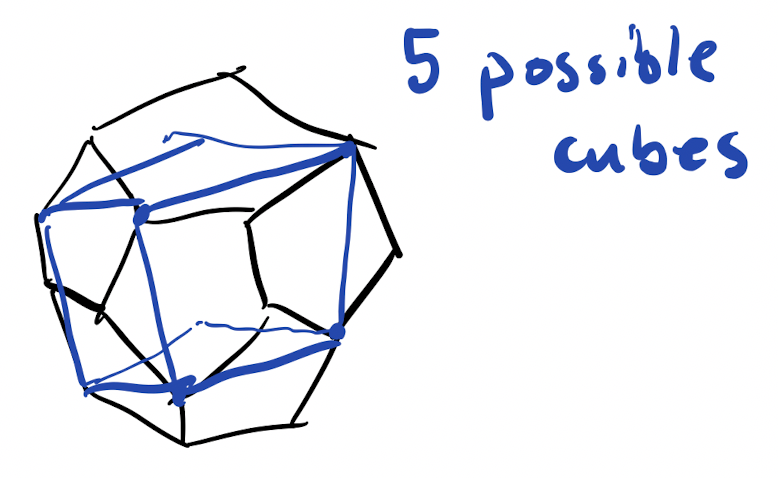
\includegraphics[width=7cm]{Lecture Files and Images/lec20-dodec.png}
\end{center}

Recall from before that $I$ is the symmetry group of both the icosahedron and the dodecahedron. There are five cubes fitting in the dodecahedron where the vertices are vertices of the dodecahedron and the edges of the cubes are diagonals of the pentagons that are the faces of the dodecahdron. For such a cube, every face of the dodecahedron will contain exactly one edge of the cube. Once one diagonal on one face is chosen, it determines the rest of the cube, and since a pentagon has five diagonals, there are 5 such cubes. 

Let $S$ be the set of $5$ cubes in the dodecahedron, labeled from 1 to 5 in some order. Then, $I$ clearly acts on $S,$ since it acts on the dodecahedron. 

Let 
\[
f: I \xrightarrow[\text{non-trivial}]{} \perm(S) = S_5
\]
take an element of $I$ to the corresponding permutation of the five cubes.

The group $I$ is simple, and the kernel of a homomorphism is always normal, so $\ker(f) \nsub I = \{e\}$ or $I.$ Since $f$ is nontrivial, $\ker(f) \neq I,$ so $\ker(f) = \{e\}.$ This implies that the homomorphism $f$ must be injective. 

Then, consider a different homomorphism $\varphi$ taking $I \rto \{\pm 1\}$, the composition
\[
I \xrightarrow[]{f} S_5 \xrightarrow[]{\text{sign}} \{\pm 1\}.
\]

Again, $\ker(\varphi) = \{e\}$ or $\ker(\varphi) = I.$ Since $|I| = 60 > |\{\pm 1\}| = 2,$ $\varphi$ is mapping a larger group onto a smaller group and cannot be injective, so $\ker(\varphi) = I.$ So under $\varphi,$ every element of $I$ maps to 1. However, this implies that the sign of the corresponding permutation of some element of $I$ is 1, so the corresponding permutation is even, and so $f(I),$ a subgroup of permutations in $S_5,$ consists entirely of even permutations. Then $f(I) \subseteq \ker(\text{sign}) = A_5,$ so $f$ is actually a homomorphism from $I$ to $A_5 \subset S_5;$ since it is injective from $I$ to $S_5,$ it is still injective from $I$ to $A_5.$ Since $I$ and $A_5$ are both of order 60, $f$ is also a surjection, and thus $f$ is an isomorphism between $I$ and $A_5$. 
\end{proof}

Throughout this proof, the fact that $I$ is simple is used over and over again to argue facts about various homomorphisms coming from $I.$

\begin{corollary}
The alternating group $A_5$ is also simple.
\end{corollary}

In fact, $A_n$ is simple for all $n \geq 5,$ but the proof is more complicated and involves thinking about the actual permutations. For the proof that $A_5$ is isomorphic to $I$ and thus simple, the class equation was the jumping-off point. The class equation showed that $I$ was simple, which then provided strong restrictions on homomorphisms from it. 

\subsection{Conjugacy Classes for Symmetric Groups}

Next time, the conjugacy classes for $S_n$ and $A_n$ will be determined. Recall that every $\sigma \in S_n$ can be decomposed via cycles. 
\begin{example}
The permutation $(123)(45) \in S_6$ takes $1 \mapsto 2,$ $2 \mapsto 3,$ and $3 \mapsto 1$ as the first cycle, of length 3, then $4 \mapsto 5$ and $5 \mapsto 4$ as the second cycle, of length 2, and $6 \mapsto 6$ as the third cycle, of length 1. 
\end{example}

The \textbf{sign} of $\sigma$, where $\sigma = \tau_1 \cdots \tau_r,$ where each $\tau_i$ is a 2-cycle\footnote{Also called a transposition.}, is $(-1)^r.$ For example, the sign of $(1234) = (12)(13)(12)$ is $-1.$ 

\newpage